%--------------
%% preamble.tex
%% this should be included with a command like
%% %--------------
%% preamble.tex
%% this should be included with a command like
%% %--------------
%% preamble.tex
%% this should be included with a command like
%% \input{preamble.tex}
%% Template based on Aleksander Madry's and Dan Spielman's template
\documentclass[12pt]{article}
%\renewcommand{\baselinestretch}{1.5}
\usepackage[OT4]{fontenc}
\newtheorem{define}{Definition}
\usepackage{amsmath}
\usepackage{graphicx}
\usepackage{enumitem}
\usepackage{float}
\usepackage{color}

\oddsidemargin=0.15in
\evensidemargin=0.15in
\topmargin=-.5in
\textheight=9in
\textwidth=6.25in

\renewcommand{\thefootnote}{\fnsymbol{footnote}}

\hbadness=10000
\vbadness=10000

%\setlength{\oddsidemargin}{.1in}
%\setlength{\evensidemargin}{.1in}
%\setlength{\textwidth}{6in}
\setlength{\topmargin}{-0.4in}
\setlength{\textheight}{8.5in}

\newcommand{\handout}[5]{
	\noindent
	\begin{center}
		\framebox{
			\vbox{
				\hbox to 5.78in { {\bf #1}
					\hfill #2 }
				\vspace{4mm}
				\hbox to 5.78in { {\Large \hfill #5  \hfill} }
				\vspace{2mm}
				\hbox to 5.78in { {\it #3 \hfill #4} }
			}
		}
	\end{center}
	\vspace*{4mm}
}

\newcommand{\header}[3]{\handout{NUS CS-CS5562: Trustworthy Machine Learning}{\today}{Lecturer: Reza Shokri}{Student: #2\quad#3}{#1}}


\newtheorem{theorem}{Theorem}
\newtheorem{corollary}[theorem]{Corollary}
\newtheorem{lemma}[theorem]{Lemma}
\newtheorem{observation}[theorem]{Observation}
\newtheorem{proposition}[theorem]{Proposition}
\newtheorem{definition}[theorem]{Definition}
\newtheorem{claim}[theorem]{Claim}
\newtheorem{fact}[theorem]{Fact}
\newtheorem{assumption}[theorem]{Assumption}

\newcommand{\qed}{\rule{7pt}{7pt}}
\newcommand{\dis}{\mathop{\mbox{\rm d}}\nolimits}
\newcommand{\per}{\mathop{\mbox{\rm per}}\nolimits}
\newcommand{\area}{\mathop{\mbox{\rm area}}\nolimits}
\newcommand{\cw}{\mathop{\rm cw}\nolimits}
\newcommand{\ccw}{\mathop{\rm ccw}\nolimits}
\newcommand{\DIST}{\mathop{\mbox{\rm DIST}}\nolimits}
\newcommand{\OP}{\mathop{\mbox{\it OP}}\nolimits}
\newcommand{\OPprime}{\mathop{\mbox{\it OP}^{\,\prime}}\nolimits}
\newcommand{\ihat}{\hat{\imath}}
\newcommand{\jhat}{\hat{\jmath}}
\newcommand{\abs}[1]{\mathify{\left| #1 \right|}}

\newenvironment{proof}{\noindent{\bf Proof}\hspace*{1em}}{\qed\bigskip}
\newenvironment{proof-sketch}{\noindent{\bf Sketch of Proof}\hspace*{1em}}{\qed\bigskip}
\newenvironment{proof-idea}{\noindent{\bf Proof Idea}\hspace*{1em}}{\qed\bigskip}
\newenvironment{proof-of-lemma}[1]{\noindent{\bf Proof of Lemma #1}\hspace*{1em}}{\qed\bigskip}
\newenvironment{proof-attempt}{\noindent{\bf Proof Attempt}\hspace*{1em}}{\qed\bigskip}
\newenvironment{proofof}[1]{\noindent{\bf Proof}
of #1:\hspace*{1em}}{\qed\bigskip}
\newenvironment{remark}{\noindent{\bf Remark}\hspace*{1em}}{\bigskip}

% \makeatletter
% \@addtoreset{figure}{section}
% \@addtoreset{table}{section}
% \@addtoreset{equation}{section}
% \makeatother

\newcommand{\FOR}{{\bf for}}
\newcommand{\TO}{{\bf to}}
\newcommand{\DO}{{\bf do}}
\newcommand{\WHILE}{{\bf while}}
\newcommand{\AND}{{\bf and}}
\newcommand{\IF}{{\bf if}}
\newcommand{\THEN}{{\bf then}}
\newcommand{\ELSE}{{\bf else}}

% \renewcommand{\thefigure}{\thesection.\arabic{figure}}
% \renewcommand{\thetable}{\thesection.\arabic{table}}
% \renewcommand{\theequation}{\thesection.\arabic{equation}}

\makeatletter
\def\fnum@figure{{\bf Figure \thefigure}}
\def\fnum@table{{\bf Table \thetable}}
\long\def\@mycaption#1[#2]#3{\addcontentsline{\csname
  ext@#1\endcsname}{#1}{\protect\numberline{\csname
  the#1\endcsname}{\ignorespaces #2}}\par
  \begingroup
    \@parboxrestore
    \small
    \@makecaption{\csname fnum@#1\endcsname}{\ignorespaces #3}\par
  \endgroup}
\def\mycaption{\refstepcounter\@captype \@dblarg{\@mycaption\@captype}}
\makeatother

\newcommand{\figcaption}[1]{\mycaption[]{#1}}
\newcommand{\tabcaption}[1]{\mycaption[]{#1}}
\newcommand{\head}[1]{\chapter[Lecture \##1]{}}
\newcommand{\mathify}[1]{\ifmmode{#1}\else\mbox{$#1$}\fi}
%\renewcommand{\Pr}[1]{\mathify{\mbox{Pr}\left[#1\right]}}
%\newcommand{\Exp}[1]{\mathify{\mbox{Exp}\left[#1\right]}}
\newcommand{\bigO}O
\newcommand{\set}[1]{\mathify{\left\{ #1 \right\}}}
\def\half{\frac{1}{2}}

\newcommand{\fig}[4]{
        \begin{figure}
        \setlength{\epsfysize}{#2}
        \vspace{3mm}
        \centerline{\epsfbox{#4}}
        \caption{#3} \label{#1}
        \end{figure}
        }

\newcommand{\ord}{{\rm ord}}

\providecommand{\norm}[1]{\lVert #1 \rVert}
\newcommand{\embed}{{\rm Embed}}
\newcommand{\qembed}{\mbox{$q$-Embed}}
\newcommand{\calh}{{\cal H}}
\newcommand{\lp}{{\rm LP}}

\newcounter{mysolctr}

\newenvironment{mysolution}% environment name
{% begin code
	\refstepcounter{mysolctr}
	\color{blue}
	\par\vspace{\baselineskip}%
	\textbf{Solution \themysolctr}%
	\par\vspace{\baselineskip}%
}%
{}% end code
\numberwithin{mysolctr}{section}

\newenvironment{pts}% environment name
{% begin code
	\color{red}
	\par\vspace{\baselineskip}%
	\textbf{Points Scheme}%
	\par\vspace{\baselineskip}%
}%
{}% end code 

%% Template based on Aleksander Madry's and Dan Spielman's template
\documentclass[12pt]{article}
%\renewcommand{\baselinestretch}{1.5}
\usepackage[OT4]{fontenc}
\newtheorem{define}{Definition}
\usepackage{amsmath}
\usepackage{graphicx}
\usepackage{enumitem}
\usepackage{float}
\usepackage{color}

\oddsidemargin=0.15in
\evensidemargin=0.15in
\topmargin=-.5in
\textheight=9in
\textwidth=6.25in

\renewcommand{\thefootnote}{\fnsymbol{footnote}}

\hbadness=10000
\vbadness=10000

%\setlength{\oddsidemargin}{.1in}
%\setlength{\evensidemargin}{.1in}
%\setlength{\textwidth}{6in}
\setlength{\topmargin}{-0.4in}
\setlength{\textheight}{8.5in}

\newcommand{\handout}[5]{
	\noindent
	\begin{center}
		\framebox{
			\vbox{
				\hbox to 5.78in { {\bf #1}
					\hfill #2 }
				\vspace{4mm}
				\hbox to 5.78in { {\Large \hfill #5  \hfill} }
				\vspace{2mm}
				\hbox to 5.78in { {\it #3 \hfill #4} }
			}
		}
	\end{center}
	\vspace*{4mm}
}

\newcommand{\header}[3]{\handout{NUS CS-CS5562: Trustworthy Machine Learning}{\today}{Lecturer: Reza Shokri}{Student: #2\quad#3}{#1}}


\newtheorem{theorem}{Theorem}
\newtheorem{corollary}[theorem]{Corollary}
\newtheorem{lemma}[theorem]{Lemma}
\newtheorem{observation}[theorem]{Observation}
\newtheorem{proposition}[theorem]{Proposition}
\newtheorem{definition}[theorem]{Definition}
\newtheorem{claim}[theorem]{Claim}
\newtheorem{fact}[theorem]{Fact}
\newtheorem{assumption}[theorem]{Assumption}

\newcommand{\qed}{\rule{7pt}{7pt}}
\newcommand{\dis}{\mathop{\mbox{\rm d}}\nolimits}
\newcommand{\per}{\mathop{\mbox{\rm per}}\nolimits}
\newcommand{\area}{\mathop{\mbox{\rm area}}\nolimits}
\newcommand{\cw}{\mathop{\rm cw}\nolimits}
\newcommand{\ccw}{\mathop{\rm ccw}\nolimits}
\newcommand{\DIST}{\mathop{\mbox{\rm DIST}}\nolimits}
\newcommand{\OP}{\mathop{\mbox{\it OP}}\nolimits}
\newcommand{\OPprime}{\mathop{\mbox{\it OP}^{\,\prime}}\nolimits}
\newcommand{\ihat}{\hat{\imath}}
\newcommand{\jhat}{\hat{\jmath}}
\newcommand{\abs}[1]{\mathify{\left| #1 \right|}}

\newenvironment{proof}{\noindent{\bf Proof}\hspace*{1em}}{\qed\bigskip}
\newenvironment{proof-sketch}{\noindent{\bf Sketch of Proof}\hspace*{1em}}{\qed\bigskip}
\newenvironment{proof-idea}{\noindent{\bf Proof Idea}\hspace*{1em}}{\qed\bigskip}
\newenvironment{proof-of-lemma}[1]{\noindent{\bf Proof of Lemma #1}\hspace*{1em}}{\qed\bigskip}
\newenvironment{proof-attempt}{\noindent{\bf Proof Attempt}\hspace*{1em}}{\qed\bigskip}
\newenvironment{proofof}[1]{\noindent{\bf Proof}
of #1:\hspace*{1em}}{\qed\bigskip}
\newenvironment{remark}{\noindent{\bf Remark}\hspace*{1em}}{\bigskip}

% \makeatletter
% \@addtoreset{figure}{section}
% \@addtoreset{table}{section}
% \@addtoreset{equation}{section}
% \makeatother

\newcommand{\FOR}{{\bf for}}
\newcommand{\TO}{{\bf to}}
\newcommand{\DO}{{\bf do}}
\newcommand{\WHILE}{{\bf while}}
\newcommand{\AND}{{\bf and}}
\newcommand{\IF}{{\bf if}}
\newcommand{\THEN}{{\bf then}}
\newcommand{\ELSE}{{\bf else}}

% \renewcommand{\thefigure}{\thesection.\arabic{figure}}
% \renewcommand{\thetable}{\thesection.\arabic{table}}
% \renewcommand{\theequation}{\thesection.\arabic{equation}}

\makeatletter
\def\fnum@figure{{\bf Figure \thefigure}}
\def\fnum@table{{\bf Table \thetable}}
\long\def\@mycaption#1[#2]#3{\addcontentsline{\csname
  ext@#1\endcsname}{#1}{\protect\numberline{\csname
  the#1\endcsname}{\ignorespaces #2}}\par
  \begingroup
    \@parboxrestore
    \small
    \@makecaption{\csname fnum@#1\endcsname}{\ignorespaces #3}\par
  \endgroup}
\def\mycaption{\refstepcounter\@captype \@dblarg{\@mycaption\@captype}}
\makeatother

\newcommand{\figcaption}[1]{\mycaption[]{#1}}
\newcommand{\tabcaption}[1]{\mycaption[]{#1}}
\newcommand{\head}[1]{\chapter[Lecture \##1]{}}
\newcommand{\mathify}[1]{\ifmmode{#1}\else\mbox{$#1$}\fi}
%\renewcommand{\Pr}[1]{\mathify{\mbox{Pr}\left[#1\right]}}
%\newcommand{\Exp}[1]{\mathify{\mbox{Exp}\left[#1\right]}}
\newcommand{\bigO}O
\newcommand{\set}[1]{\mathify{\left\{ #1 \right\}}}
\def\half{\frac{1}{2}}

\newcommand{\fig}[4]{
        \begin{figure}
        \setlength{\epsfysize}{#2}
        \vspace{3mm}
        \centerline{\epsfbox{#4}}
        \caption{#3} \label{#1}
        \end{figure}
        }

\newcommand{\ord}{{\rm ord}}

\providecommand{\norm}[1]{\lVert #1 \rVert}
\newcommand{\embed}{{\rm Embed}}
\newcommand{\qembed}{\mbox{$q$-Embed}}
\newcommand{\calh}{{\cal H}}
\newcommand{\lp}{{\rm LP}}

\newcounter{mysolctr}

\newenvironment{mysolution}% environment name
{% begin code
	\refstepcounter{mysolctr}
	\color{blue}
	\par\vspace{\baselineskip}%
	\textbf{Solution \themysolctr}%
	\par\vspace{\baselineskip}%
}%
{}% end code
\numberwithin{mysolctr}{section}

\newenvironment{pts}% environment name
{% begin code
	\color{red}
	\par\vspace{\baselineskip}%
	\textbf{Points Scheme}%
	\par\vspace{\baselineskip}%
}%
{}% end code 

%% Template based on Aleksander Madry's and Dan Spielman's template
\documentclass[12pt]{article}
%\renewcommand{\baselinestretch}{1.5}
\usepackage[OT4]{fontenc}
\newtheorem{define}{Definition}
\usepackage{amsmath}
\usepackage{graphicx}
\usepackage{enumitem}
\usepackage{float}
\usepackage{color}

\oddsidemargin=0.15in
\evensidemargin=0.15in
\topmargin=-.5in
\textheight=9in
\textwidth=6.25in

\renewcommand{\thefootnote}{\fnsymbol{footnote}}

\hbadness=10000
\vbadness=10000

%\setlength{\oddsidemargin}{.1in}
%\setlength{\evensidemargin}{.1in}
%\setlength{\textwidth}{6in}
\setlength{\topmargin}{-0.4in}
\setlength{\textheight}{8.5in}

\newcommand{\handout}[5]{
	\noindent
	\begin{center}
		\framebox{
			\vbox{
				\hbox to 5.78in { {\bf #1}
					\hfill #2 }
				\vspace{4mm}
				\hbox to 5.78in { {\Large \hfill #5  \hfill} }
				\vspace{2mm}
				\hbox to 5.78in { {\it #3 \hfill #4} }
			}
		}
	\end{center}
	\vspace*{4mm}
}

\newcommand{\header}[3]{\handout{NUS CS-CS5562: Trustworthy Machine Learning}{\today}{Lecturer: Reza Shokri}{Student: #2\quad#3}{#1}}


\newtheorem{theorem}{Theorem}
\newtheorem{corollary}[theorem]{Corollary}
\newtheorem{lemma}[theorem]{Lemma}
\newtheorem{observation}[theorem]{Observation}
\newtheorem{proposition}[theorem]{Proposition}
\newtheorem{definition}[theorem]{Definition}
\newtheorem{claim}[theorem]{Claim}
\newtheorem{fact}[theorem]{Fact}
\newtheorem{assumption}[theorem]{Assumption}

\newcommand{\qed}{\rule{7pt}{7pt}}
\newcommand{\dis}{\mathop{\mbox{\rm d}}\nolimits}
\newcommand{\per}{\mathop{\mbox{\rm per}}\nolimits}
\newcommand{\area}{\mathop{\mbox{\rm area}}\nolimits}
\newcommand{\cw}{\mathop{\rm cw}\nolimits}
\newcommand{\ccw}{\mathop{\rm ccw}\nolimits}
\newcommand{\DIST}{\mathop{\mbox{\rm DIST}}\nolimits}
\newcommand{\OP}{\mathop{\mbox{\it OP}}\nolimits}
\newcommand{\OPprime}{\mathop{\mbox{\it OP}^{\,\prime}}\nolimits}
\newcommand{\ihat}{\hat{\imath}}
\newcommand{\jhat}{\hat{\jmath}}
\newcommand{\abs}[1]{\mathify{\left| #1 \right|}}

\newenvironment{proof}{\noindent{\bf Proof}\hspace*{1em}}{\qed\bigskip}
\newenvironment{proof-sketch}{\noindent{\bf Sketch of Proof}\hspace*{1em}}{\qed\bigskip}
\newenvironment{proof-idea}{\noindent{\bf Proof Idea}\hspace*{1em}}{\qed\bigskip}
\newenvironment{proof-of-lemma}[1]{\noindent{\bf Proof of Lemma #1}\hspace*{1em}}{\qed\bigskip}
\newenvironment{proof-attempt}{\noindent{\bf Proof Attempt}\hspace*{1em}}{\qed\bigskip}
\newenvironment{proofof}[1]{\noindent{\bf Proof}
of #1:\hspace*{1em}}{\qed\bigskip}
\newenvironment{remark}{\noindent{\bf Remark}\hspace*{1em}}{\bigskip}

% \makeatletter
% \@addtoreset{figure}{section}
% \@addtoreset{table}{section}
% \@addtoreset{equation}{section}
% \makeatother

\newcommand{\FOR}{{\bf for}}
\newcommand{\TO}{{\bf to}}
\newcommand{\DO}{{\bf do}}
\newcommand{\WHILE}{{\bf while}}
\newcommand{\AND}{{\bf and}}
\newcommand{\IF}{{\bf if}}
\newcommand{\THEN}{{\bf then}}
\newcommand{\ELSE}{{\bf else}}

% \renewcommand{\thefigure}{\thesection.\arabic{figure}}
% \renewcommand{\thetable}{\thesection.\arabic{table}}
% \renewcommand{\theequation}{\thesection.\arabic{equation}}

\makeatletter
\def\fnum@figure{{\bf Figure \thefigure}}
\def\fnum@table{{\bf Table \thetable}}
\long\def\@mycaption#1[#2]#3{\addcontentsline{\csname
  ext@#1\endcsname}{#1}{\protect\numberline{\csname
  the#1\endcsname}{\ignorespaces #2}}\par
  \begingroup
    \@parboxrestore
    \small
    \@makecaption{\csname fnum@#1\endcsname}{\ignorespaces #3}\par
  \endgroup}
\def\mycaption{\refstepcounter\@captype \@dblarg{\@mycaption\@captype}}
\makeatother

\newcommand{\figcaption}[1]{\mycaption[]{#1}}
\newcommand{\tabcaption}[1]{\mycaption[]{#1}}
\newcommand{\head}[1]{\chapter[Lecture \##1]{}}
\newcommand{\mathify}[1]{\ifmmode{#1}\else\mbox{$#1$}\fi}
%\renewcommand{\Pr}[1]{\mathify{\mbox{Pr}\left[#1\right]}}
%\newcommand{\Exp}[1]{\mathify{\mbox{Exp}\left[#1\right]}}
\newcommand{\bigO}O
\newcommand{\set}[1]{\mathify{\left\{ #1 \right\}}}
\def\half{\frac{1}{2}}

\newcommand{\fig}[4]{
        \begin{figure}
        \setlength{\epsfysize}{#2}
        \vspace{3mm}
        \centerline{\epsfbox{#4}}
        \caption{#3} \label{#1}
        \end{figure}
        }

\newcommand{\ord}{{\rm ord}}

\providecommand{\norm}[1]{\lVert #1 \rVert}
\newcommand{\embed}{{\rm Embed}}
\newcommand{\qembed}{\mbox{$q$-Embed}}
\newcommand{\calh}{{\cal H}}
\newcommand{\lp}{{\rm LP}}

\newcounter{mysolctr}

\newenvironment{mysolution}% environment name
{% begin code
	\refstepcounter{mysolctr}
	\color{blue}
	\par\vspace{\baselineskip}%
	\textbf{Solution \themysolctr}%
	\par\vspace{\baselineskip}%
}%
{}% end code
\numberwithin{mysolctr}{section}

\newenvironment{pts}% environment name
{% begin code
	\color{red}
	\par\vspace{\baselineskip}%
	\textbf{Points Scheme}%
	\par\vspace{\baselineskip}%
}%
{}% end code 

\usepackage{hyperref}
\usepackage{booktabs}
\usepackage{comment}
\usepackage{bbm}
\usepackage{mathtools}
\usepackage{amsfonts}
\usepackage{appendix}
\usepackage{csquotes}
\usepackage{amssymb}
\usepackage{listings}
\usepackage{float}
\usepackage{amsmath}
\lstset{
    frame = single,
    breaklines=true,
    basicstyle=\ttfamily}
\usepackage{tikz, forest}
\usepackage[square,numbers]{natbib}
\bibliographystyle{abbrvnat}

\DeclareMathOperator*{\maximize}{maximize}
\DeclareMathOperator*{\minimize}{minimize}


\begin{document}

% Indicate your name and your student number (e.g., A01xxx)
\header{Assignment 4}{Niharika Shrivastava}{A0245355A}

\section*{2 Private Training via DP-SGD}
\subsection*{2.1 DP-SGD}

\begin{table}[h]
    \centering
    \begin{tabular}{| c | c | c |}
        \hline
        Model & Train Accuracy & Test Accuracy\\
        \hline 
        Non-Private & 83.51 & 82.52\\
        \hline
        Private & 84.22 & 82.39\\
        \hline
    \end{tabular}
\end{table}

The test accuracy for the private model decreased compared to the non-private model, i.e., the utility for the private model decreased at the cost of increased privacy.

\subsection*{2.2 Computing Privacy Parameters of DP-SGD using Moments Accountant}

Given,

\begin{table}[htp]
    \centering
    \begin{tabular}{|c|c|c|c|c|c|c|c|}
    \hline
        Parameter & $\sigma$ & B & 
        E & N & $\delta$ & q & T \\
        \hline
        Value & 0.05 & 1 & 20 & $10^4$ & $10^{-5}$ & $B/N = 10^{-4}$ & $E \times N = 2 \times 10^5$ \\
        \hline
    \end{tabular}
    \caption{Caption}
    \label{tab:my_label}
\end{table}

By Theorem 2.2 (Tail bound) in \cite{abadi},
$$ \delta = \min_\lambda e^{[\alpha(\lambda) - \lambda\epsilon]} $$
$$ \frac{\partial \delta}{\partial \lambda} = e^{[\alpha(\lambda) - \lambda\epsilon]}[\frac{\partial \alpha(\lambda)}{\partial \lambda} - \epsilon] = 0 $$
$$ \Rightarrow \frac{\partial \alpha(\lambda)}{\partial \lambda} = \epsilon $$

By Theorem 2.1 and Lemma 3 in \cite{abadi}, the log moment of DP-SGD can be bounded as follows:
$$ \alpha(\lambda) \leq T q^2\lambda^2 / \sigma^2 $$
$$ \frac{\partial \alpha(\lambda)}{\partial \lambda} \leq \frac{2Tq^2 \lambda}{\sigma^2} \Rightarrow \epsilon \leq \frac{2Tq^2 \lambda}{\sigma^2} $$

By Theorem 2 in \cite{abadi}, to guarantee DP-SGD to be ($\epsilon$, $\delta$)-differentially private, it suffices that:
$$ \epsilon \geq \frac{2Tq^2 \lambda}{\sigma^2} $$
$$ \Rightarrow \epsilon = \frac{2Tq^2 \lambda}{\sigma^2}, \alpha(\lambda) = E q^2\lambda^2 / \sigma^2 $$

By substituting the value of $\epsilon$ and $\alpha(\lambda)$,
$$ \lambda = \sqrt{\frac{-\sigma^2 \log \delta}{Tq^2}} = 3.7935 $$
$$ \epsilon = 6.0967 $$


\subsection*{2.3 Effect of Clipping Norm on Accuracy}

\begin{enumerate}
    \item The $l_2$ norm trajectory of the privatized gradients is much noisier than the true gradients since we add Gaussian noise in each epoch. Thus, the gradient descent is not smooth.
    
    \begin{figure}[h]
        \centering
        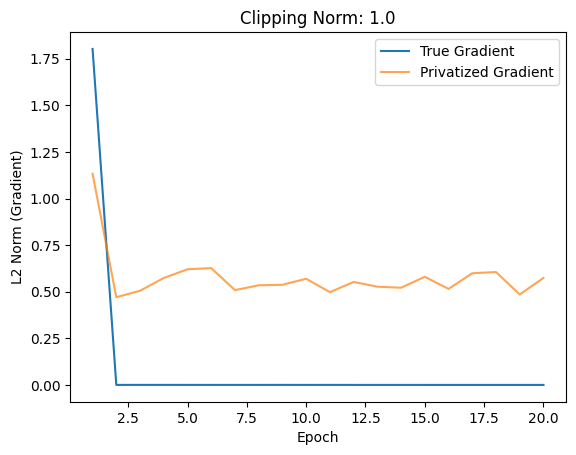
\includegraphics[width=0.5\linewidth]{report/images/quest2-3-1.png}
        \caption{Question 2.3.1}
        \label{fig:enter-label}
    \end{figure}

    \item As the clipping norm increases, the magnitude of the private gradients increases and they become increasingly jagged. This is because the standard deviation of the noise added to the gradients is linearly proportional to C.

    \begin{tabular}{c c c c}
        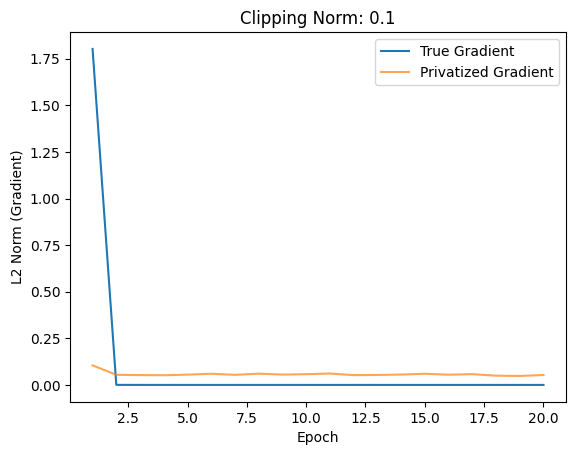
\includegraphics[width=3.5cm]{report/images/1.png} & 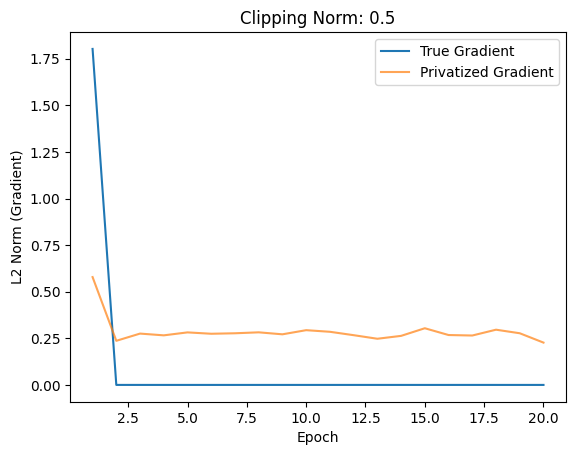
\includegraphics[width=3.5cm]{report/images/2.png} & 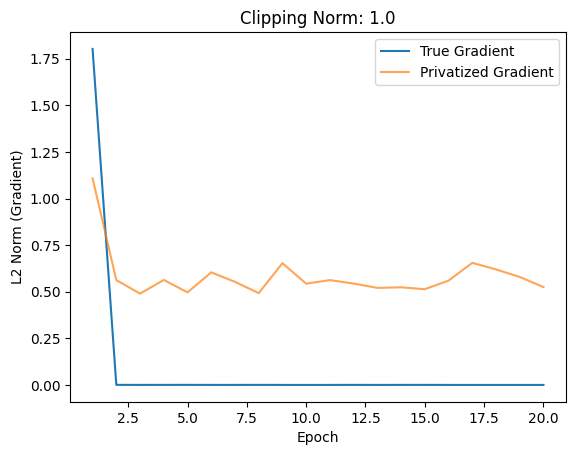
\includegraphics[width=3.5cm]{report/images/3.png} & 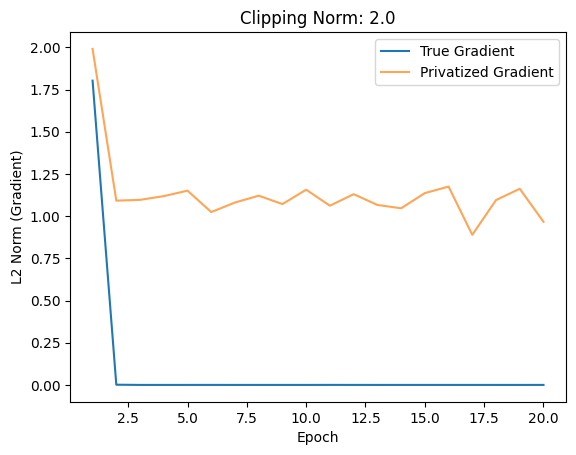
\includegraphics[width=3.5cm]{report/images/4.png} \\
    \end{tabular}

    \item As the clipping norm C increases, the accuracy of the model decreases. This is because the amount of noise added to the gradients increases with increasing clipping norm which lowers the accuracy.

    \begin{figure}[h]
        \centering
        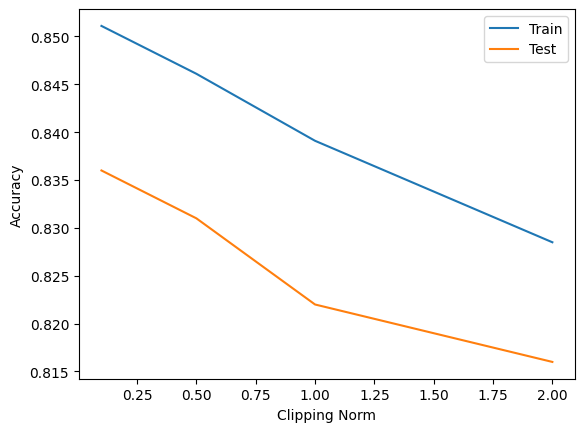
\includegraphics[width=0.5\linewidth]{report/images/quest2-3-2.png}
        \caption{Question 2.3.2}
        \label{fig:enter-label}
    \end{figure}
    
\end{enumerate}

\section*{3 Membership inference on DP models}

\subsection*{3.1 Theorem Proof}

From the definition of $(\epsilon, \delta)$-differential privacy, 
$$ Pr[Y=y | X=x] \leq e^\epsilon \cdot Pr[Y=y|X=x'] + \delta $$
where $ x = D \bigcup z, x' = D $.

\begin{itemize}
    \item $Pr[Y=y | X=x]$ means that the attacker correctly predicts that $z \in x$, i.e., the True Positive Rate (TPR).

    \item $Pr[Y = y|X = x']$ means that the attacker wrongly predicts that $z \in x'$, i.e., the False Positive Rate (FPR).
\end{itemize}

Thus, by rewriting the definition as follows:

$$ TPR \leq e^\epsilon \cdot FPR + \delta $$
$$ \Rightarrow e^\epsilon \cdot FPR + (1 - TPR) \geq 1 - \delta  $$

Similarly, we can rewrite the definition of DP as follows:
$$ Pr[Y \neq y | X=x'] \leq e^\epsilon \cdot Pr[Y \neq y|X=x] + \delta $$

\begin{itemize}
    \item $Pr[Y \neq y | X=x']$ means that the attacker correctly predicts that $z \notin x'$, i.e., the True Negative Rate (TNR).

    \item $Pr[Y \neq y|X = x]$ means that the attacker wrongly predicts that $z \notin x$, i.e., the False Negative Rate (FNR).
\end{itemize}

Thus, by rewriting the definition as follows:

$$ TNR \leq e^\epsilon \cdot FNR + \delta $$
$$ 1 - FPR \leq e^\epsilon \cdot (1-TPR) + \delta $$
$$ \Rightarrow e^\epsilon \cdot (1-TPR) + FPR \geq 1 - \delta  $$

\subsection*{Plotting}

\begin{itemize}
    \item The TPR, FPR values for distinguishing two histograms satisfy the inequalities in Theorem 1. Moreover, this membership inference attack is so poor that it is almost indistinguishable to infer membership even in the worst-case scenario.
    
    However, the bounds of our DP-SGD are too loose. The AUC is almost 1. This means that $\sigma = 0.05$ is not enough to make our algorithm a good differentially private algorithm.
    \begin{figure}[htp]
        \centering
        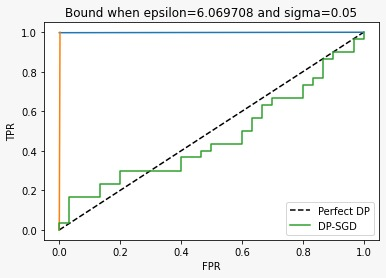
\includegraphics[width=0.5\linewidth]{report//images/quest3.jpeg}
    \end{figure}

    \item For a higher noise multiplier, $\epsilon$ would be lesser and the bounds would be much tighter, thereby making it a better defense algorithm. 
\end{itemize}



\bibliography{report/refs}

\end{document}
